\chapter{系统内核}\label{ch:system-kernel}

\section{系统内核简介}\label{sec:kernel-introduction}

的内核提供了一个可使用的实时操作系统应具有的最简单的功能，主要包括线程、线程延时、邮箱机制和信号量机制。如果用户需要更复杂的机制，那么可以从提供的几种基本机制出发实现其他的机制。本系统还额外提供了一个轻量级图形界面库，它在不使用\footnote{未检测到相关宏被定义}的时候完全不消耗内存。

本系统推荐用于32个优先级以下，64个线程以下的系统。本系统理论上最多支持的线程数量和优先级数量都是无限的，但为了系统效率和易用性，不推荐使用本系统实现超过这个复杂度的嵌入式应用。如果需要实现更复杂的嵌入式应用，推荐使用0等更高级的系统。

\subsection{内核调度器}\label{subsec:kernel-scheduler}

内核的调度器是一个全抢占式的固定优先级时间片轮转的调度器。该类调度器在同一个优先级内部使用时间片轮转法则进行线程调度，在不同的优先级之间则采取抢占式调度策略。和某些RTOS不同，的调度器在某些架构上永远不会关闭中断，从而保证了系统的实时性。为了提高内核的实时性，当处理器具备、等指令时，还可以使用这些指令加速最高优先级查找。

没有\footnote{将来也永远不会}内建对多核系统的直接支持。如果要支持多核处理器也是可能的，这需要编译多个副本并且在每个处理器上运行一个副本，以分区操作系统的方式存在，类似于\hyperref[sec:chapter-bibliography-4]{{[}1{]}}。

\subsection{内存管理与内存保护}\label{subsec:memory-management-and-memory-protection}

提供了一个基于二级分割适配算法（Two-Level Segregated Fit,
TLSF）\hyperref[sec:chapter-bibliography-4]{{[}2{]}{[}3{]}}机制的内存分配器。这个分配器在所有O(1)时间复杂度的内存分配器中具备较高空间效率。然而，在小型嵌入式系统中动态内存分配并不被推荐，因此应该尽量少用该分配器。不具备真正意义上的内存保护功能，各个线程之间的地址是没有隔离的，因此在编写应用程序时应当遵循编程规范。

\subsection{应用升级与应用模块}\label{subsec:application-updating-and-application-modules}

由于本系统相对较为小型，因此不支持应用升级和应用模块。通常而言，使用本系统编译出的完整映像大小不应超过128kB，因此是可以全部升级的。如果需要应用模块功能，那么需要用户自行实现。

\subsection{系统启动流程}\label{subsec:system-boot-sequence}

RMP内核的第一个线程永远是RMP\_Init，它位于内核提供的代码中。RMP\_Init线程负责系统的初期初始化和低功耗，并且它永远不可能停止运行。RMP\_Init线程引出了两个钩子RMP\_Init\_Hook和RMP\_Init\_Idle，它们负责将用户代码导入到内核运行的过程中。关于这两个接口的说明请参见第\ref{subsec:mandatory-hook-interface}节所述。

\section{线程调度接口}\label{sec:thread-scheduling-interface}

由于整个系统都运行在一个地址空间，因此系统仅提供线程抽象。线程可以有就绪、运行、悬起、阻塞\footnote{包括延时、等待信号量、等待邮箱接收、等待邮箱发送四种基本阻塞方式}四种状态，阻塞状态还具有一段时间后接收不到自动返回的功能。悬起状态可以被施加于任何线程，此时该线程总是暂时停止执行，无论其当前处于什么状态。

完整的线程状态转移图如下所示：

\begin{figure}[htbp]
    \centering
    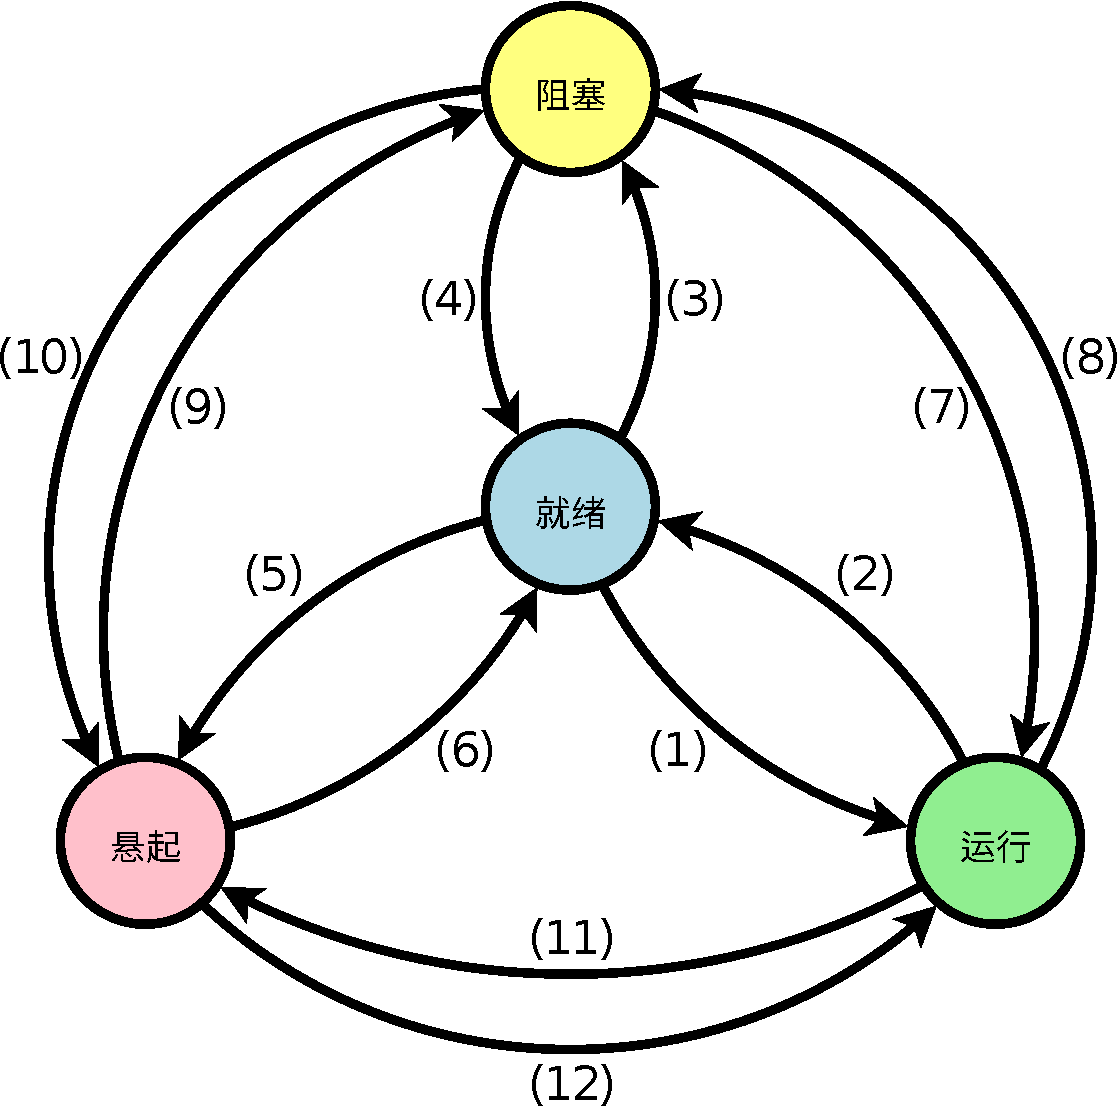
\includegraphics[width=0.72\textwidth]{Figure/thread_state_cn.pdf}
    \caption{线程状态转移图}
    \label{fig:thread-state-transition-diagram}
\end{figure}

图中各个数字标号的意义如下所示：

\captionof{table}{线程状态转移图中各标号的含义}\label{tab:meaning-of-the-labels-in-the-thread-state-transition-diagram}

{\def\LTcaptype{none} % do not increment counter
\begin{longtable}[]{@{}
  >{\raggedright\arraybackslash}p{(\linewidth - 2\tabcolsep) * \real{0.0750}}
  >{\raggedright\arraybackslash}p{(\linewidth - 2\tabcolsep) * \real{0.9250}}@{}}
\toprule\noalign{}
\begin{minipage}[b]{\linewidth}\raggedright
标号
\end{minipage} & \begin{minipage}[b]{\linewidth}\raggedright
代表意义
\end{minipage} \\
\midrule\noalign{}
\endhead
\bottomrule\noalign{}
\endlastfoot
(1) & 该线程处于就绪态且优先级最高，因此由就绪态转入运行态。 \\
(2) & 该线程处于运行态且优先级非最高，因此由运行态转入就绪态。 \\
(3) &
该可能性不存在（图中以虚线表示），线程不可能直接由就绪态进入阻塞态。 \\
(4) &
该线程被解除阻塞且未悬起，且优先级非最高，因此由阻塞态进入就绪态。 \\
(5) & 该线程在就绪态被悬起，因此由就绪态进入悬起态。 \\
(6) &
该线程被解除悬起且未阻塞，且优先级非最高，因此由悬起态进入就绪态。 \\
(7) &
该线程被解除阻塞且未悬起，且优先级最高，因此由阻塞态进入运行态。 \\
(8) & 该线程在邮箱、信号量或延时功能处阻塞，因此由运行态进入阻塞态。 \\
(9) & 该线程在被解除悬起且仍在阻塞，因此由悬起态进入阻塞态。 \\
(10) & 该线程在阻塞态被悬起，因此由阻塞态进入悬起态。 \\
(11) & 该线程在运行态被悬起，因此由运行态进入悬起态。 \\
(12) &
该线程在被解除悬起且未阻塞，且优先级最高，因此由悬起态进入运行态。 \\
\end{longtable}
}

所有的线程调度接口如下表所示：

\captionof{table}{线程调度接口一览}\label{tab:thread-scheduling-interface-summary}

{\def\LTcaptype{none} % do not increment counter
\begin{longtable}[]{@{}
  >{\raggedright\arraybackslash}p{(\linewidth - 6\tabcolsep) * \real{0.3210}}
  >{\raggedright\arraybackslash}p{(\linewidth - 6\tabcolsep) * \real{0.3146}}
  >{\raggedright\arraybackslash}p{(\linewidth - 6\tabcolsep) * \real{0.1759}}
  >{\raggedright\arraybackslash}p{(\linewidth - 6\tabcolsep) * \real{0.1817}}@{}}
\toprule\noalign{}
\begin{minipage}[b]{\linewidth}\raggedright
接口
\end{minipage} & \begin{minipage}[b]{\linewidth}\raggedright
意义
\end{minipage} & \begin{minipage}[b]{\linewidth}\raggedright
锁调度器时调用
\end{minipage} & \begin{minipage}[b]{\linewidth}\raggedright
中断中调用
\end{minipage} \\
\midrule\noalign{}
\endhead
\bottomrule\noalign{}
\endlastfoot
RMP\_Thd\_Crt & 创建线程 & 可 & 不可 \\
RMP\_Thd\_Del & 删除线程 & 可 & 不可 \\
RMP\_Thd\_Set & 设置线程属性 & 可 & 不可 \\
RMP\_Thd\_Yield & 出让处理器 &
不可\footnotemark{} & 不可 \\
RMP\_Thd\_Suspend & 悬起线程 & 不可 & 不可 \\
RMP\_Thd\_Resume & 解除线程悬起 & 可 & 不可 \\
RMP\_Thd\_Delay & 线程延时 & 不可 & 不可 \\
RMP\_Thd\_Cancel & 解除线程延时 & 可 & 不可 \\
RMP\_Thd\_Loop & 线程循环延时 & 可 & 不可 \\
\end{longtable}
}
\footnotetext{不可能阻塞当前线程的操作均可在锁调度器时调用，但可能会阻塞或出让当前线程的操作则不可在锁调度器时调用；这个标准同样适用于后面各章节中列出的接口}

它们可能有如下返回值：

\captionof{table}{线程调度接口的可能返回值}\label{tab:possible-return-values-of-the-thread-scheduling-interface}

{\def\LTcaptype{none} % do not increment counter
\begin{longtable}[]{@{}
  >{\raggedright\arraybackslash}p{(\linewidth - 4\tabcolsep) * \real{0.2741}}
  >{\raggedright\arraybackslash}p{(\linewidth - 4\tabcolsep) * \real{0.0927}}
  >{\raggedright\arraybackslash}p{(\linewidth - 4\tabcolsep) * \real{0.6332}}@{}}
\toprule\noalign{}
\begin{minipage}[b]{\linewidth}\raggedright
返回值
\end{minipage} & \begin{minipage}[b]{\linewidth}\raggedright
数值
\end{minipage} & \begin{minipage}[b]{\linewidth}\raggedright
意义
\end{minipage} \\
\midrule\noalign{}
\endhead
\bottomrule\noalign{}
\endlastfoot
RMP\_ERR\_THD & -1 & 由于线程控制块相关的原因导致操作失败。 \\
RMP\_ERR\_PRIO & -2 & 由于优先级相关的原因导致操作失败。 \\
RMP\_ERR\_SLICE & -3 & 由于时间片相关的原因导致操作失败。 \\
RMP\_ERR\_STACK & -4 & 由于运行栈相关的原因导致操作失败。 \\
RMP\_ERR\_STATE & -5 & 由于线程状态相关的原因导致操作失败。 \\
RMP\_ERR\_OPER & -6 & 由于其他原因导致操作失败。 \\
\end{longtable}
}

具体的各个函数中返回值的意义请在相应函数下查找。

\subsection{创建线程}\label{subsec:create-a-thread}

本操作会创建一个新的线程并使其处于就绪态。新创建的线程总是会被插入到同优先级时间片轮转队列的末尾：如果没有其它干扰，则先创建的线程总是先被调度。

\begin{apidesc}{RMP\_Thd\_Crt}{创建线程}
    \apisig{rmp\_ret\_t RMP\_Thd\_Crt(volatile struct RMP\_Thd* Thread, void* Entry, void* Param, void* Stack, rmp\_ptr\_t Size, rmp\_ptr\_t Prio, rmp\_ptr\_t Slice)}
    \begin{apiparams}
        \apiparam{volatile struct RMP\_Thd* Thread}{指向空的、将被用于该线程的线程控制块的指针。}
        \apiparam{void* Entry}{线程的入口地址。}
        \apiparam{void* Param}{传递给线程的参数。}
        \apiparam{void* Stack}{线程的运行栈的起始地址。如果以数组的形式分配它，则此处填写数组的首地址。某些架构对栈的内存地址有特殊要求\footnote{如必须位于地址空间的低64KiB等；如果涉及堆栈段寄存器，请参见\ref{subsubsec:the-common-memory-model-is-the-small-model}}，此时该地址必须满足这些要求。}
        \apiparam{rmp\_ptr\_t Size}{线程的运行栈的大小，单位为字节。如果以数组的形式分配它，则此处填写数组的大小。}
        \apiparam{rmp\_ptr\_t Prio}{线程的优先级。在本系统中，优先级数字越大，优先级越高。}
        \apiparam{rmp\_ptr\_t Slice}{线程的时间片数量。时间片数量的单位是时钟嘀嗒。}
    \end{apiparams}
    当 \texttt{RMP\_STKSEG\_ENABLE} 非 0 时，\texttt{Param} 与 \texttt{Stack} 之间还有一个 \texttt{rmp\_ptr\_t Segment} 参数，用于指定线程的堆栈段。
    \begin{apiret}
        \apiretval{rmp\_ret\_t}{如果成功，返回0。如果失败则可能有如下返回值：}
        \apiretval{RMP\_ERR\_STACK}{输入的栈区域为0（NULL）或者栈大小放不下上下文。}
        \apiretval{RMP\_ERR\_PRIO}{输入的优先级不小于RMP\_PREEMPT\_PRIO\_NUM。}
        \apiretval{RMP\_ERR\_SLICE}{输入的时间片为0或不小于RMP\_SLICE\_MAX。}
        \apiretval{RMP\_ERR\_THD}{线程控制块为0（NULL）或者正在被使用。}
    \end{apiret}
\end{apidesc}

\subsection{删除线程}\label{subsec:delete-a-thread}

本操作会删除系统中的一个线程。线程被删除后，一切资源将释放，正在向它发送的线程的发送等待将被解除并会返回发送失败。

值得注意的是，的线程并不允许通过返回来直接退出。如果任何一个线程想要终止自己，就必须显式调用这个函数删除自己。这个设计是有意而为，是为了显式地提醒用户线程正被删除，从而方便用户最大限度地避免``创建
- 运行一次 -
删除''的用法\footnote{这种用法应该被``阻塞 - 运行一次 - 再次阻塞''或线程池技术代替}。

\begin{apidesc}{RMP\_Thd\_Del}{删除线程}
    \apisig{rmp\_ret\_t RMP\_Thd\_Del(volatile struct RMP\_Thd* Thread)}
    \begin{apiparams}
        \apiparam{volatile struct RMP\_Thd* Thread}{指向要删除的线程的线程控制块的指针。}
    \end{apiparams}
    \begin{apiret}
        \apiretval{rmp\_ret\_t}{如果成功，返回0。如果失败则可能有如下返回值：}
        \apiretval{RMP\_ERR\_THD}{线程控制块为0（NULL）或者未被使用。}
    \end{apiret}
\end{apidesc}

\subsection{设置线程属性}\label{subsec:set-thread-attributes}

本操作会设置某个线程的时间片和优先级。当只需要设置其中一个时，只要保证另一个参数是RMP\_PREEMPT\_PRIO\_NUM或RMP\_SLICE\_MAX即可。

\begin{apidesc}{RMP\_Thd\_Set}{设置线程属性}
    \apisig{rmp\_ret\_t RMP\_Thd\_Set(volatile struct RMP\_Thd* Thread, rmp\_ptr\_t Prio, rmp\_ptr\_t Slice)}
    \begin{apiparams}
        \apiparam{volatile struct RMP\_Thd* Thread}{指向要更改优先级和时间片的线程的线程控制块的指针。}
        \apiparam{rmp\_ptr\_t Prio}{要设置的优先级。输入RMP\_PREEMPT\_PRIO\_NUM代表不修改优先级。 在本系统中，优先级数字越大，优先级越高。}
        \apiparam{rmp\_ptr\_t Slice}{要设置的时间片数量。输入RMP\_SLICE\_MAX代表不修改时间片。}
    \end{apiparams}
    \begin{apiret}
        \apiretval{rmp\_ret\_t}{如果成功，返回0。如果失败则可能有如下返回值：}
        \apiretval{RMP\_ERR\_PRIO}{输入的优先级大于RMP\_PREEMPT\_PRIO\_NUM。}
        \apiretval{RMP\_ERR\_SLICE}{输入的时间片为0或者大于RMP\_SLICE\_MAX。}
        \apiretval{RMP\_ERR\_THD}{线程控制块为0（NULL）或者未被使用。}
    \end{apiret}
\end{apidesc}

\subsection{出让处理器}\label{subsec:yield-the-processor}

本操作会使当前线程放弃CPU，并且调度器会自动选择下一个线程进行调度。如果当前线程的优先级是最高的，且那个优先级上只有它，那么它仍然会被调度。

\begin{apidesc}{RMP\_Thd\_Yield}{出让处理器}
    \apisig{void RMP\_Thd\_Yield(void)}
    \begin{apiparams}
        \apiparam{无。}{}
    \end{apiparams}
    \begin{apiret}
        \apiretval{无。}{}
    \end{apiret}
\end{apidesc}

\subsection{悬起线程}\label{subsec:suspend-a-thread}

本操作会使某线程悬起，使调度器暂时停止对其的调度。无论线程处于哪个状态，它都可以被悬起，但是已经处于的延时、发送、接收等状态仍继续存在，也即线程处于悬起状态和延时、发送、接收等状态之一的叠加。当延时、发送、接收等状态结束后，如果该线程还处于被悬起状态，那么它将被置于纯粹的悬起状态，仍然不参与调度，直到悬起状态被手动解除。

\begin{apidesc}{RMP\_Thd\_Suspend}{悬起线程}
    \apisig{rmp\_ret\_t RMP\_Thd\_Suspend(volatile struct RMP\_Thd* Thread)}
    \begin{apiparams}
        \apiparam{volatile struct RMP\_Thd* Thread}{指向要悬起执行的线程的线程控制块的指针。}
    \end{apiparams}
    \begin{apiret}
        \apiretval{rmp\_ret\_t}{如果成功，返回0。如果失败则可能有如下返回值：}
        \apiretval{RMP\_ERR\_THD}{线程控制块为0（NULL）或者未被使用。}
        \apiretval{RMP\_ERR\_STATE}{该线程已经被悬起，无法被再次悬起。 该检查即使在关闭时也会执行。}
    \end{apiret}
\end{apidesc}

\subsection{解除线程悬起}\label{subsec:resume-a-suspended-thread}

本操作会解除某个线程的悬起状态，使其有重新参与调度的可能。

\begin{apidesc}{RMP\_Thd\_Resume}{解除线程悬起}
    \apisig{rmp\_ret\_t RMP\_Thd\_Resume(volatile struct RMP\_Thd* Thread)}
    \begin{apiparams}
        \apiparam{volatile struct RMP\_Thd* Thread}{指向要解除悬起的线程的线程控制块的指针。}
    \end{apiparams}
    \begin{apiret}
        \apiretval{rmp\_ret\_t}{如果成功，返回0。如果失败则可能有如下返回值：}
        \apiretval{RMP\_ERR\_THD}{线程控制块为0（NULL）或者未被使用。}
        \apiretval{RMP\_ERR\_STATE}{该线程未被悬起，无法被解除悬起。 该检查即使在关闭时也会执行。}
    \end{apiret}
\end{apidesc}

\subsection{线程延时}\label{subsec:delay-a-thread}

本操作会使当前线程延时一段时间。

\begin{apidesc}{RMP\_Thd\_Delay}{线程延时}
    \apisig{rmp\_ret\_t RMP\_Thd\_Delay(rmp\_ptr\_t Slice)}
    \begin{apiparams}
        \apiparam{rmp\_ptr\_t Slice}{要延时的时间，单位是时间片。}
    \end{apiparams}
    \begin{apiret}
        \apiretval{rmp\_ret\_t}{如果成功，返回0。如果失败则可能有如下返回值：}
        \apiretval{RMP\_ERR\_SLICE}{输入的时间片为0或不小于RMP\_SLICE\_MAX。}
        \apiretval{RMP\_ERR\_OPER}{该延时没有进行完毕就被解除。 该检查即使在关闭时也会执行。}
    \end{apiret}
\end{apidesc}

\subsection{解除线程延时}\label{subsec:cancel-a-thread-delay}

本操作会解除某个线程的延时。

\begin{apidesc}{RMP\_Thd\_Cancel}{解除线程延时}
    \apisig{rmp\_ret\_t RMP\_Thd\_Cancel(volatile struct RMP\_Thd* Thread)}
    \begin{apiparams}
        \apiparam{volatile struct RMP\_Thd* Thread}{指向要解除延时的线程的线程控制块的指针。}
    \end{apiparams}
    \begin{apiret}
        \apiretval{rmp\_ret\_t}{如果成功，返回0。如果失败则可能有如下返回值：}
        \apiretval{RMP\_ERR\_THD}{线程控制块为0（NULL）或者未被使用。}
        \apiretval{RMP\_ERR\_STATE}{该线程未处于延时状态，无法被解除延时。 该检查即使在关闭时也会执行。}
    \end{apiret}
\end{apidesc}

\subsection{线程循环延时}\label{subsec:thread-busy-wait}

本操作会使当前线程陷入死循环一段时间。与其它线程接口不同，它可以在锁调度器或者关中断的条件下使用，且延时粒度精细，但会白白浪费处理器性能。

\begin{apidesc}{RMP\_Thd\_Loop}{线程循环延时}
    \apisig{void RMP\_Thd\_Loop(rmp\_ptr\_t Loop)}
    \begin{apiparams}
        \apiparam{rmp\_ptr\_t Loop}{要延时的时间，单位是循环数。循环数和处理器周期之间的换算可能随不同的处理器、工具链和优化等级而有不同。}
    \end{apiparams}
    \begin{apiret}
        \apiretval{无。}{}
    \end{apiret}
\end{apidesc}

\subsection{从中断窥探接替线程}\label{subsec:peek-at-the-next-thread-from-an-isr}

本操作可用来在中断或调度器锁定中窥探即将接替当前线程执行的线程。如果系统中没有发生可以解除线程阻塞的事件，则接替当前线程的就是本函数返回的线程。作为特例，如果当前线程是系统中最高优先级的就绪线程，且这个优先级上除当前线程之外还有其它线程就绪，本操作将返回当前线程的下一个线程，也即若在此刻调用时将选中的那个线程。

这个操作的主要用途是在那些低优先级线程的使用调度器锁的长临界区中定期探测是否有高优先级线程就绪；如果有，低优先级线程可以提前放弃调度器锁以减少中断延迟。

\begin{apidesc}{RMP\_Thd\_Peek\_ISR}{从中断窥探接替线程}
    \apisig{volatile struct RMP\_Thd* RMP\_Thd\_Peek\_ISR(void)}
    \begin{apiparams}
        \apiparam{无。}{}
    \end{apiparams}
    \begin{apiret}
        \apiretval{volatile struct RMP\_Thd*}{指向接替线程的线程控制块的指针。}
    \end{apiret}
\end{apidesc}

\section{线程邮箱和信号量接口}\label{sec:thread-mailbox-and-semaphore-interface}

提供了简单而高效的线程间通信机制，包括线程邮箱（Mailbox）和信号量（Semaphore），其中信号量是带操作计数、排队等待、阻塞解锁和批量唤醒的，因而既可作为线程间的条件变量和计数器又可作为线程内的锁。上述两个基本机制可以被单独使用，也可以被组合成更复杂的通信接口使用。可以阻塞的通信接口都有三个选项：探知可能阻塞后立即返回、阻塞超时后返回、一直阻塞。这大大提高了接口使用的灵活性。需要注意的是，所有的通信接口在有多个线程阻塞时，服务顺序永远是按照时间先后顺序的，不提供优先级插队功能。如果一个高优先级线程在低优先级线程阻塞后才阻塞，那么第一个被服务的是低优先级线程，然后才是高优先级线程。

所有的线程邮箱和信号量接口如下表所示：

\captionof{table}{线程邮箱和信号量接口一览}\label{tab:thread-mailbox-and-semaphore-interface-summary}

{\def\LTcaptype{none} % do not increment counter
\begin{longtable}[]{@{}
  >{\raggedright\arraybackslash}p{(\linewidth - 6\tabcolsep) * \real{0.3210}}
  >{\raggedright\arraybackslash}p{(\linewidth - 6\tabcolsep) * \real{0.3146}}
  >{\raggedright\arraybackslash}p{(\linewidth - 6\tabcolsep) * \real{0.1759}}
  >{\raggedright\arraybackslash}p{(\linewidth - 6\tabcolsep) * \real{0.1817}}@{}}
\toprule\noalign{}
\begin{minipage}[b]{\linewidth}\raggedright
接口
\end{minipage} & \begin{minipage}[b]{\linewidth}\raggedright
意义
\end{minipage} & \begin{minipage}[b]{\linewidth}\raggedright
锁调度器时调用
\end{minipage} & \begin{minipage}[b]{\linewidth}\raggedright
中断中调用
\end{minipage} \\
\midrule\noalign{}
\endhead
\bottomrule\noalign{}
\endlastfoot
RMP\_Thd\_Snd & 向线程邮箱发送 & 不可 & 不可 \\
RMP\_Thd\_Snd\_ISR & 在中断中向线程邮箱发送 & 不可 & 可 \\
RMP\_Thd\_Rcv & 从线程邮箱接收 & 不可 & 不可 \\
RMP\_Sem\_Crt & 创建信号量 & 可 & 不可 \\
RMP\_Sem\_Del & 删除信号量 & 可 & 不可 \\
RMP\_Sem\_Post & 发布信号量 & 可 & 不可 \\
RMP\_Sem\_Post\_ISR & 从中断发布信号量 & 不可 & 可 \\
RMP\_Sem\_Bcst & 广播信号量 & 可 & 不可 \\
RMP\_Sem\_Bcst\_ISR & 从中断广播信号量 & 不可 & 可 \\
RMP\_Sem\_Pend & 等待信号量 & 不可 & 不可 \\
RMP\_Sem\_Pend\_Unlock & 等待信号量并解除调度器锁 & 可，仅单层锁 &
不可 \\
RMP\_Sem\_Abort & 解除信号量等待 & 可 & 不可 \\
RMP\_Sem\_Cnt & 查询信号量数目 & 可 & 不可 \\
\end{longtable}
}

它们可能有如下返回值：

\captionof{table}{线程邮箱和信号量接口的可能返回值}\label{tab:possible-return-values-of-the-thread-mailbox-and-semaphore-interface}

{\def\LTcaptype{none} % do not increment counter
\begin{longtable}[]{@{}
  >{\raggedright\arraybackslash}p{(\linewidth - 4\tabcolsep) * \real{0.2741}}
  >{\raggedright\arraybackslash}p{(\linewidth - 4\tabcolsep) * \real{0.0927}}
  >{\raggedright\arraybackslash}p{(\linewidth - 4\tabcolsep) * \real{0.6332}}@{}}
\toprule\noalign{}
\begin{minipage}[b]{\linewidth}\raggedright
返回值
\end{minipage} & \begin{minipage}[b]{\linewidth}\raggedright
数值
\end{minipage} & \begin{minipage}[b]{\linewidth}\raggedright
意义
\end{minipage} \\
\midrule\noalign{}
\endhead
\bottomrule\noalign{}
\endlastfoot
RMP\_ERR\_THD & -1 & 由于线程控制块相关的原因导致操作失败。 \\
RMP\_ERR\_SLICE & -3 & 由于时间片相关的原因导致操作失败。 \\
RMP\_ERR\_STATE & -5 & 由于线程状态相关的原因导致操作失败。 \\
RMP\_ERR\_OPER & -6 & 由于其他原因导致操作失败。 \\
RMP\_ERR\_SEM & -7 & 由于信号量控制块相关的原因导致操作失败。 \\
\end{longtable}
}

\subsection{向线程邮箱发送}\label{subsec:send-to-a-thread-mailbox}

本操作会向线程邮箱发送一个处理器字长的信息。

\begin{apidesc}{RMP\_Thd\_Snd}{向线程邮箱发送}
    \apisig{rmp\_ret\_t RMP\_Thd\_Snd(volatile struct RMP\_Thd* Thread, rmp\_ptr\_t Data, rmp\_ptr\_t Slice)}
    \begin{apiparams}
        \apiparam{volatile struct RMP\_Thd* Thread}{指向要发送到的线程的线程控制块的指针。}
        \apiparam{rmp\_ptr\_t Data}{要发送的数据。}
        \apiparam{rmp\_ptr\_t Slice}{要等待的时间片数量。如果为0，那么意味着如果探测到阻塞则立即返回；如果为0到RMP\_SLICE\_MAX之间的值，那么将会最多阻塞等待该数量的时间片后返回；如果为超过或等于RMP\_SLICE\_MAX的值，那么意味着将永远阻塞直到被接收或者目标线程被销毁。}
    \end{apiparams}
    \begin{apiret}
        \apiretval{rmp\_ret\_t}{如果成功，返回0。如果失败则可能有如下返回值：}
        \apiretval{RMP\_ERR\_THD}{线程控制块为0（NULL）或者未被使用。}
        \apiretval{RMP\_ERR\_OPER}{在不阻塞条件下探测到可能造成阻塞，或者试图发送到自己的邮箱，或者发送因超时、目标线程被删除而失败。 最后一条检查即使在关闭时也会执行。}
    \end{apiret}
\end{apidesc}

\subsection{在中断中向线程邮箱发送}\label{subsec:send-to-a-thread-mailbox-from-an-interrupt}

本操作会从中断向量中向线程邮箱发送一个处理器字长的信息。和上面的普通版本调用不同，该版本总是立即返回而不会阻塞。

\begin{apidesc}{RMP\_Thd\_Snd\_ISR}{在中断中向线程邮箱发送}
    \apisig{rmp\_ret\_t RMP\_Thd\_Snd\_ISR(volatile struct RMP\_Thd* Thread, rmp\_ptr\_t Data)}
    \begin{apiparams}
        \apiparam{volatile struct RMP\_Thd* Thread}{指向要发送到的线程的线程控制块的指针。}
        \apiparam{rmp\_ptr\_t Data}{要发送的数据。}
    \end{apiparams}
    \begin{apiret}
        \apiretval{rmp\_ret\_t}{如果成功，返回0。如果失败则可能有如下返回值：}
        \apiretval{RMP\_ERR\_THD}{线程控制块为0（NULL）或者未被使用。}
        \apiretval{RMP\_ERR\_OPER}{目标线程的邮箱已满，无法发送。 该检查即使在关闭时也会执行。}
    \end{apiret}
\end{apidesc}

\subsection{从线程邮箱接收}\label{subsec:receive-from-a-thread-mailbox}

本操作会从当前线程的邮箱中接收一个处理器字长的值。

\begin{apidesc}{RMP\_Thd\_Rcv}{从线程邮箱接收}
    \apisig{rmp\_ret\_t RMP\_Thd\_Rcv(rmp\_ptr\_t* Data, rmp\_ptr\_t Slice)}
    \begin{apiparams}
        \apiparam{rmp\_ptr\_t* Data}{该参数用于输出，输出接收到的数据。如果传入RMP\_NULL，则接收到的数据会被丢弃。}
        \apiparam{rmp\_ptr\_t Slice}{要等待的时间片数量。如果为0，那么意味着如果探测到阻塞则立即返回；如果为0到RMP\_SLICE\_MAX之间的值，那么将会最多阻塞等待该数量的时间片后返回；如果为超过或等于RMP\_SLICE\_MAX的值，那么意味着将永远阻塞直到接收完成。}
    \end{apiparams}
    \begin{apiret}
        \apiretval{rmp\_ret\_t}{如果成功，返回0。如果失败则可能有如下返回值：}
        \apiretval{RMP\_ERR\_OPER}{在不阻塞条件下探测到可能造成阻塞，或者接收因超时而失败。 该检查即使在关闭时也会执行。}
    \end{apiret}
\end{apidesc}

\subsection{创建信号量}\label{subsec:create-a-semaphore}

本操作会创建一个新的信号量。

\begin{apidesc}{RMP\_Sem\_Crt}{创建信号量}
    \apisig{rmp\_ret\_t RMP\_Sem\_Crt(volatile struct RMP\_Sem* Semaphore, rmp\_ptr\_t Number)}
    \begin{apiparams}
        \apiparam{volatile struct RMP\_Sem* Semaphore}{指向空的、将被用于该信号量的信号量控制块的指针。}
        \apiparam{rmp\_ptr\_t Number}{该信号量的初始值，应该小于RMP\_SEM\_CNT\_MAX。}
    \end{apiparams}
    \begin{apiret}
        \apiretval{rmp\_ret\_t}{如果成功，返回0。如果失败则可能有如下返回值：}
        \apiretval{RMP\_ERR\_SEM}{信号量控制块为0（NULL）或者已被使用。}
        \apiretval{RMP\_ERR\_OPER}{初始信号量值过大，超过或等于RMP\_SEM\_CNT\_MAX。}
    \end{apiret}
\end{apidesc}

\subsection{删除信号量}\label{subsec:delete-a-semaphore}

本操作会删除一个信号量。
如果有线程在其上阻塞，那么这些线程的等待信号量函数会直接返回。

\begin{apidesc}{RMP\_Sem\_Del}{删除信号量}
    \apisig{rmp\_ret\_t RMP\_Sem\_Del(volatile struct RMP\_Sem* Semaphore)}
    \begin{apiparams}
        \apiparam{volatile struct RMP\_Sem* Semaphore}{指向要删除的信号量的信号量控制块的指针。}
    \end{apiparams}
    \begin{apiret}
        \apiretval{rmp\_ret\_t}{如果成功，返回0。如果失败则可能有如下返回值：}
        \apiretval{RMP\_ERR\_SEM}{信号量控制块为0（NULL）或者未被使用。}
    \end{apiret}
\end{apidesc}

\subsection{发布信号量}\label{subsec:post-to-a-semaphore}

本操作会发布一定数量的信号到某信号量。

\begin{apidesc}{RMP\_Sem\_Post}{发布信号量}
    \apisig{rmp\_ret\_t RMP\_Sem\_Post(volatile struct RMP\_Sem* Semaphore, rmp\_ptr\_t Number)}
    \begin{apiparams}
        \apiparam{volatile struct RMP\_Sem* Semaphore}{指向要发布到的信号量的信号量控制块的指针。}
        \apiparam{rmp\_ptr\_t Number}{要发布的信号数量。}
    \end{apiparams}
    \begin{apiret}
        \apiretval{rmp\_ret\_t}{如果成功，返回0。如果失败则可能有如下返回值：}
        \apiretval{RMP\_ERR\_SEM}{信号量控制块为0（NULL）或者未被使用。}
        \apiretval{RMP\_ERR\_OPER}{欲发布的数量为0，或者目标信号量如果接受此数量的信号会溢出（超过或等于RMP\_SEM\_CNT\_MAX）。}
    \end{apiret}
\end{apidesc}

\subsection{从中断发布信号量}\label{subsec:post-to-a-semaphore-from-an-interrupt}

本操作会从中断中发布一定数量的信号到某信号量。

\begin{apidesc}{RMP\_Sem\_Post\_ISR}{从中断发布信号量}
    \apisig{rmp\_ret\_t RMP\_Sem\_Post\_ISR(volatile struct RMP\_Sem* Semaphore, rmp\_ptr\_t Number)}
    \begin{apiparams}
        \apiparam{volatile struct RMP\_Sem* Semaphore}{指向要发布到的信号量的信号量控制块的指针。}
        \apiparam{rmp\_ptr\_t Number}{要发布的信号数量。}
    \end{apiparams}
    \begin{apiret}
        \apiretval{rmp\_ret\_t}{如果成功，返回0。如果失败则可能有如下返回值：}
        \apiretval{RMP\_ERR\_SEM}{信号量控制块为0（NULL）或者未被使用。}
        \apiretval{RMP\_ERR\_OPER}{欲发布的数量为0，或者目标信号量如果接受此数量的信号会溢出（超过或等于RMP\_SEM\_CNT\_MAX）。}
    \end{apiret}
\end{apidesc}

\subsection{广播信号量}\label{subsec:broadcast-a-semaphore}

本操作会发布足够数量的信号到某信号量，使其上面的一切等待线程解除阻塞。如果该信号量上无线程阻塞，则不会发送任何信号。

\begin{apidesc}{RMP\_Sem\_Bcst}{广播信号量}
    \apisig{rmp\_ret\_t RMP\_Sem\_Bcst(volatile struct RMP\_Sem* Semaphore)}
    \begin{apiparams}
        \apiparam{volatile struct RMP\_Sem* Semaphore}{指向要广播到的信号量的信号量控制块的指针。}
    \end{apiparams}
    \begin{apiret}
        \apiretval{rmp\_ret\_t}{如果成功，返回成功解除阻塞的线程的数量。如果失败则可能有如下返回值：}
        \apiretval{RMP\_ERR\_SEM}{信号量控制块为0（NULL）或者未被使用。}
    \end{apiret}
\end{apidesc}

\subsection{从中断广播信号量}\label{subsec:broadcast-a-semaphore-from-an-interrupt}

本操作会发布足够数量的信号到某信号量，使其上面的一切等待线程解除阻塞。如果该信号量上无线程阻塞，则不会发送任何信号。使用本操作可能导致一次解除大量线程的阻塞，从而造成中断执行超期；使用时必须加以注意。

\begin{apidesc}{RMP\_Sem\_Bcst\_ISR}{从中断广播信号量}
    \apisig{rmp\_ret\_t RMP\_Sem\_Bcst\_ISR(volatile struct RMP\_Sem* Semaphore)}
    \begin{apiparams}
        \apiparam{volatile struct RMP\_Sem* Semaphore}{指向要广播到的信号量的信号量控制块的指针。}
    \end{apiparams}
    \begin{apiret}
        \apiretval{rmp\_ret\_t}{如果成功，返回成功解除阻塞的线程的数量。如果失败则可能有如下返回值：}
        \apiretval{RMP\_ERR\_SEM}{信号量控制块为0（NULL）或者未被使用。}
    \end{apiret}
\end{apidesc}

\subsection{等待信号量}\label{subsec:wait-on-a-semaphore}

本操作会使当前线程尝试获取信号量。获取的数量总是为1。

\begin{apidesc}{RMP\_Sem\_Pend}{等待信号量}
    \apisig{rmp\_ret\_t RMP\_Sem\_Pend(volatile struct RMP\_Sem* Semaphore, rmp\_ptr\_t Slice)}
    \begin{apiparams}
        \apiparam{volatile struct RMP\_Sem* Semaphore}{指向要等待的信号量的信号量控制块的指针。}
        \apiparam{rmp\_ptr\_t Slice}{暂无信号量时要等待的时间片数量。如果为0，那么意味着如果探测到阻塞则立即返回；如果为0到RMP\_SLICE\_MAX之间的值，那么将会最多阻塞等待该数量的时间片后返回；如果为超过或等于RMP\_SLICE\_MAX的值，那么意味着将永远阻塞直到获取到信号量或者目标信号量被销毁。}
    \end{apiparams}
    \begin{apiret}
        \apiretval{rmp\_ret\_t}{如果成功，返回当前信号量的剩余值。如果失败则可能有如下返回值：}
        \apiretval{RMP\_ERR\_SEM}{信号量控制块为0（NULL）或者未被使用。}
        \apiretval{RMP\_ERR\_OPER}{在不阻塞条件下探测到可能造成阻塞，或者等待因超时、目标信号量被删除、被中途解除而失败。 该检查即使在RMP\_CHECK\_ENABLE关闭时也会执行。}
    \end{apiret}
\end{apidesc}

\subsection{等待信号量并解除调度器锁}\label{subsec:wait-on-a-semaphore-and-unlock-the-scheduler}

本操作与等待信号量是类似的，其唯一区别是在调用它之前调度器必须不多不少地上一次锁。该调用无论成败，在返回时都会解除调度器锁，相当于``等待信号量''和``解除调度器锁''的原子化合并。这在实现复杂的客制化条件变量时很有用处。

\begin{apidesc}{RMP\_Sem\_Pend\_Unlock}{等待信号量并解除调度器锁}
    \apisig{rmp\_ret\_t RMP\_Sem\_Pend\_Unlock(volatile struct RMP\_Sem* Semaphore, rmp\_ptr\_t Slice)}
    \begin{apiparams}
        \apiparam{volatile struct RMP\_Sem* Semaphore}{指向要等待的信号量的信号量控制块的指针。}
        \apiparam{rmp\_ptr\_t Slice}{暂无信号量时要等待的时间片数量。如果为0，那么意味着如果探测到阻塞则立即返回；如果为0到RMP\_SLICE\_MAX之间的值，那么将会最多阻塞等待该数量的时间片后返回；如果为超过或等于RMP\_SLICE\_MAX的值，那么意味着将永远阻塞直到获取到信号量或者目标信号量被销毁。}
    \end{apiparams}
    \begin{apiret}
        \apiretval{rmp\_ret\_t}{如果成功，返回当前信号量的剩余值。如果失败则可能有如下返回值：}
        \apiretval{RMP\_ERR\_SEM}{信号量控制块为0（NULL）或者未被使用。}
        \apiretval{RMP\_ERR\_OPER}{调度器没有正确上锁，或者在不阻塞条件下探测到可能造成阻塞，或者等待因超时、目标信号量被删除、被中途解除而失败。 最后两条检查即使在关闭时也会执行。}
    \end{apiret}
\end{apidesc}

\subsection{解除信号量等待}\label{subsec:abort-a-semaphore-wait}

本操作解除某线程的信号量等待。如果等待成功被解除，那么目标线程的等待信号量函数会返回。这个操作也同样可以用来解除消息队列与阻塞消息队列的等待，那些被解除等待的函数一样会返回RMP\_ERR\_OPER。

\begin{apidesc}{RMP\_Sem\_Abort}{解除信号量等待}
    \apisig{rmp\_ret\_t RMP\_Sem\_Abort(volatile struct RMP\_Thd* Thread)}
    \begin{apiparams}
        \apiparam{volatile struct RMP\_Thd* Thread}{指向要取消信号量等待的线程的线程控制块的指针。}
    \end{apiparams}
    \begin{apiret}
        \apiretval{rmp\_ret\_t}{如果成功，返回0。如果失败则可能有如下返回值：}
        \apiretval{RMP\_ERR\_THD}{线程控制块为0（NULL）或者未被使用。}
        \apiretval{RMP\_ERR\_STATE}{该线程未处于等待信号量状态，无法被解除等待。 该检查即使在RMP\_CHECK\_ENABLE关闭时也会执行。}
    \end{apiret}
\end{apidesc}

\subsection{查询信号量数目}\label{subsec:query-a-semaphore-count}

本操作会查询信号量的当前数目。

\begin{apidesc}{RMP\_Sem\_Cnt}{查询信号量数目}
    \apisig{rmp\_ret\_t RMP\_Sem\_Cnt(volatile struct RMP\_Sem* Semaphore)}
    \begin{apiparams}
        \apiparam{volatile struct RMP\_Sem* Semaphore}{指向要查询数目的信号量的信号量控制块的指针。}
    \end{apiparams}
    \begin{apiret}
        \apiretval{rmp\_ret\_t}{如果成功，返回当前信号量数目。如果失败则可能有如下返回值：}
        \apiretval{RMP\_ERR\_SEM}{信号量控制块为0（NULL）或者未被使用。}
    \end{apiret}
\end{apidesc}

\section{内存管理接口}\label{sec:memory-management-interface}

提供了一个基于的内存分配器。它可以有效地管理动态内存。分配器是一种二级适配算法，它把内存块先按照2的方次放入不同的初级指数区间（First-Level
Interval，FLI），如127-64 Byte，255-128
Byte等，然后在每个区间之内再将内存块放入各个线性区间，比如在127-64
Byte的二级线性区间（Second-Level Interval，SLI）就有{[}127,
112{]}，{[}111, 96{]}，\ldots\ldots，{[}79,
64{]}一共8个。在分配时，先查找某大小对应的SLI的下一级SLI有没有可供分配的内存块，如果有则分配；如果没有则向上查找到最近的SLI，从那里分配内存。当内存被释放时，内存块会被即刻合并并且放入对应的SLI，准备下次分配。

在的实现中，FLI的数目会根据内存池的大小决定，SLI的数目则固定为8，同时规定当FLI为0时对应127-64
Byte的内存块，并且单个内存池的大小不能低于1024个机器字\footnote{对于16位机不能少于2kB，对于32位机则不能少于4kB；若少于此数量，则无使用内存池的必要}。该分配器是为128
MiB以下的内存池特别优化的，不推荐将其用于更大的内存池。此外，内存池和内存池的大小均要求对其到机器字，并且一次分配的最小内存数量为64
Byte。

内存池和线程的对应关系是非常复杂的，可以是一对一、一对多、多对一或多对多。为了最大化单线程场景下的性能，的内存管理接口不提供多线程安全性，这一点和其他内核接口非常不同。如果需要多线程安全性，可配合调度器锁或信号量自行实现。此外，不可在被分配的内存区域外进行读写，否则可能会破坏分配器的数据结构而导致异常。

所有的内存管理接口如下表所示：

\captionof{table}{内存管理接口一览}\label{tab:memory-management-interface-summary}

{\def\LTcaptype{none} % do not increment counter
\begin{longtable}[]{@{}
  >{\raggedright\arraybackslash}p{(\linewidth - 4\tabcolsep) * \real{0.3207}}
  >{\raggedright\arraybackslash}p{(\linewidth - 4\tabcolsep) * \real{0.3142}}
  >{\raggedright\arraybackslash}p{(\linewidth - 4\tabcolsep) * \real{0.3572}}@{}}
\toprule\noalign{}
\begin{minipage}[b]{\linewidth}\raggedright
接口
\end{minipage} & \begin{minipage}[b]{\linewidth}\raggedright
意义
\end{minipage} & \begin{minipage}[b]{\linewidth}\raggedright
特殊说明
\end{minipage} \\
\midrule\noalign{}
\endhead
\bottomrule\noalign{}
\endlastfoot
RMP\_Mem\_Init & 初始化内存池 &
\multirow{4}{=}{内存池管理接口不提供任何线程安全性。多线程互斥操作必须由应用程序保证，这可以通过附加调度器锁或信号量解决。} \\
RMP\_Malloc & 从内存池分配内存 \\
RMP\_Free & 向内存池归还内存 \\
RMP\_Realloc & 重新配置内存大小 \\
\end{longtable}
}

除之外，它们可能返回的唯一返回值为（-8）。

\subsection{初始化内存池}\label{subsec:initialise-a-memory-pool}

本操作按照传入的内存池大小和地址初始化该内存池。内存池的大小和地址必须对齐到机器字。

\begin{apidesc}{RMP\_Mem\_Init}{初始化内存池}
    \apisig{rmp\_ret\_t RMP\_Mem\_Init(volatile void* Pool, rmp\_ptr\_t Size)}
    \begin{apiparams}
        \apiparam{volatile void* Pool}{指向要初始化为内存池的空白内存的指针。}
        \apiparam{rmp\_ptr\_t Size}{该块空白内存的大小。}
    \end{apiparams}
    \begin{apiret}
        \apiretval{rmp\_ret\_t}{如果成功，返回0。如果失败则可能有如下返回值：}
        \apiretval{RMP\_ERR\_MEM}{内存池为空（NULL）或大小、地址未对齐，或者传入的内存池大小小于1024个机器字。}
    \end{apiret}
\end{apidesc}

\subsection{从内存池分配内存}\label{subsec:allocate-from-a-memory-pool}

本操作会试图从某内存池分配内存。分配的最小数量为64
Byte，如果试图分配的数量小于它而大于0，则实际上会分配64
Byte；如果传入的大小为0则会直接返回分配失败\footnote{该检查在关闭时会被忽略}。

\begin{apidesc}{RMP\_Malloc}{从内存池分配内存}
    \apisig{void* RMP\_Malloc(volatile void* Pool, rmp\_ptr\_t Size)}
    \begin{apiparams}
        \apiparam{volatile void* Pool}{指向要分配内存的内存池的指针。}
        \apiparam{rmp\_ptr\_t Size}{要分配的内存块大小，单位是Byte。}
    \end{apiparams}
    \begin{apiret}
        \apiretval{void*}{如果成功，指向返回内存的非0（NULL）指针。如果失败则返回0（NULL）。}
    \end{apiret}
\end{apidesc}

\subsection{向内存池归还内存}\label{subsec:return-memory-to-a-memory-pool}

本操作会向某个内存池归还内存。必须是由返回的某个尚未被归还的地址，并且必须归还到分配该内存时使用的内存池\footnote{这些检查在关闭时会被忽略}，否则该操作会安静地失败。如果为NULL，则不做任何操作。

\begin{apidesc}{RMP\_Free}{向内存池归还内存}
    \apisig{void RMP\_Free(volatile void* Pool, void* Mem\_Ptr)}
    \begin{apiparams}
        \apiparam{volatile void* Pool}{指向要归还内存的内存池的指针。}
        \apiparam{void* Mem\_Ptr}{指向要归还的内存块的指针。}
    \end{apiparams}
    \begin{apiret}
        \apiretval{无。}{}
    \end{apiret}
\end{apidesc}

\subsection{重新配置内存大小}\label{subsec:resize-a-memory-block}

本操作会试图重新配置某内存块的大小。必须是由RMP\_Malloc返回的某个尚未被归还的地址，而且传入的内存池必须与调用RMP\_Malloc时的内存池一致\footnote{这些检查在RMP\_CHECK\_ENABLE关闭时会被忽略}。该函数在成功时，会返回原内存块或者一个前Size字节和原地址内容相同的新内存块，且在大于0而小于64时默认分配64
Byte；若不成功，则返回0（NULL）且原内存块不受影响。另外，如果的值为0，该函数的行为与相同，会直接释放该内存块\footnote{这和某些的实现可能不一致}；如果为NULL，该函数的行为与相同，会直接分配新的内存块。

\begin{apidesc}{RMP\_Realloc}{重新配置内存大小}
    \apisig{void* RMP\_Realloc(volatile void* Pool, void* Mem\_Ptr, rmp\_ptr\_t Size)}
    \begin{apiparams}
        \apiparam{volatile void* Pool}{指向要重新配置大小的内存块所在的内存池的指针。}
        \apiparam{void* Mem\_Ptr}{指向要重新配置大小的内存块的指针。}
        \apiparam{rmp\_ptr\_t Size}{要将该内存块重新配置为的大小。该大小可以大于或者小于原内存块大小。}
    \end{apiparams}
    \begin{apiret}
        \apiretval{void*}{如果成功，返回指向重新配置大小后的内存块的非0（NULL）指针。如果失败则返回0（NULL）。}
    \end{apiret}
\end{apidesc}

\section{钩子函数接口}\label{sec:hook-function-interface}

为了方便在系统运行的一些关键点插入用户所需的功能，RMP系统还提供了钩子函数。钩子函数可以分为必要钩子和可选钩子两类：前者被声明成函数且必须提供，后者则被声明成宏且可不填充。

\subsection{必要钩子接口}\label{subsec:mandatory-hook-interface}

必须由用户实现的钩子函数如下：

\subsubsection{空闲线程首次运行钩子}\label{subsubsec:idle-thread-first-run-hook}

该钩子函数会在空闲线程首次运行时被调用一次。其典型用法是创建其它线程、信号量和消息队列，或者做一些系统初始化工作。需要注意的是，该钩子全程在关中断的条件下执行，因此不能调用任何可能依赖中断的操作，或者开中断的操作。如果需要调用这些操作，请在其它线程中执行。

\begin{apidesc}{RMP\_Init\_Hook}{空闲线程首次运行钩子}
    \apisig{void RMP\_Init\_Hook(void)}
    \begin{apiparams}
        \apiparam{无。}{}
    \end{apiparams}
    \begin{apiret}
        \apiretval{无。}{}
    \end{apiret}
\end{apidesc}

\subsubsection{空闲线程反复运行钩子}\label{subsubsec:idle-thread-repeated-run-hook}

该钩子函数会在空闲线程被运行时反复被调用。其典型用法是在进入低功耗模式以省电，或者做一些性能分析、堆栈检测打印输出。不可以在该钩子中使空闲线程进入阻塞状态，否则系统会崩溃。

\begin{apidesc}{RMP\_Init\_Idle}{空闲线程反复运行钩子}
    \apisig{void RMP\_Init\_Idle(void)}
    \begin{apiparams}
        \apiparam{无。}{}
    \end{apiparams}
    \begin{apiret}
        \apiretval{无。}{}
    \end{apiret}
\end{apidesc}

\subsection{可选钩子接口}\label{subsec:optional-hook-interface}

可以由用户在需要时选择性实现的钩子宏如下：

\subsubsection{系统启动钩子}\label{subsubsec:system-start-hook}

该钩子宏若被定义，则会在系统完成处理器初始化后立即被调用。由于每个移植在系统启动时都仅仅会初始化一部分最基本的硬件，因此推荐将硬件的进一步初始化放置在这个钩子内部完成。如果所想要的基本系统配置与该平台中的配置头文件提供的基本初始化冲突\footnote{比如想要配置系统到完全不同的工作频率}，那么也可以在该钩子内部重新完成系统基本配置。

\begin{apidesc}{RMP\_START\_HOOK}{系统启动钩子}
    \apisig{void RMP\_START\_HOOK(void)}
    \begin{apiparams}
        \apiparam{无。}{}
    \end{apiparams}
    \begin{apiret}
        \apiretval{无。}{}
    \end{apiret}
\end{apidesc}

\subsubsection{系统上下文保存钩子}\label{subsubsec:system-context-save-hook}

该钩子宏若被定义，则会在系统完成基本上下文保存后被调用。如果有额外的上下文\footnote{FPU和其他外设寄存器组}需要保存，可以在该函数中将这些上下文压栈。具体的实现方法请参见第四章。

\begin{apidesc}{RMP\_CTX\_SAVE}{系统上下文保存钩子}
    \apisig{void RMP\_CTX\_SAVE(void)}
    \begin{apiparams}
        \apiparam{无。}{}
    \end{apiparams}
    \begin{apiret}
        \apiretval{无。}{}
    \end{apiret}
\end{apidesc}

\subsubsection{系统上下文恢复钩子}\label{subsubsec:system-context-restore-hook}

该钩子宏若被定义，则会在系统完成基本上下文恢复前被调用。如果有额外的上下文\footnote{FPU和其他外设寄存器组}需要恢复，可以在该函数中将这些上下文弹栈。具体的实现方法请参见第四章。

\begin{apidesc}{RMP\_CTX\_LOAD}{系统上下文恢复钩子}
    \apisig{void RMP\_CTX\_LOAD(void)}
    \begin{apiparams}
        \apiparam{无。}{}
    \end{apiparams}
    \begin{apiret}
        \apiretval{无。}{}
    \end{apiret}
\end{apidesc}

\subsubsection{调度器钩子}\label{subsubsec:scheduler-hook}

该钩子宏若被定义，则会在系统完成当前线程选择时被调用。如果需要实现无嘀嗒内核，可以在这个钩子内调用相关函数进行。具体的无嘀嗒系统实现方法请参见\ref{subsec:implementation-of-a-tickless-kernel}
。

\begin{apidesc}{RMP\_SCHED\_HOOK}{调度器钩子}
    \apisig{void RMP\_SCHED\_HOOK(void)}
    \begin{apiparams}
        \apiparam{无。}{}
    \end{apiparams}
    \begin{apiret}
        \apiretval{无。}{}
    \end{apiret}
\end{apidesc}

\subsubsection{系统嘀嗒钩子}\label{subsubsec:system-tick-hook}

该钩子宏若被定义，则会在系统嘀嗒到来时被调用。

\begin{apidesc}{RMP\_TIM\_HOOK}{系统嘀嗒钩子}
    \apisig{void RMP\_TIM\_HOOK(rmp\_ptr\_t Slice)}
    \begin{apiparams}
        \apiparam{rmp\_ptr\_t Slice}{该钩子在被调用时接受的Slice参数。}
    \end{apiparams}
    \begin{apiret}
        \apiretval{无。}{}
    \end{apiret}
\end{apidesc}

\subsubsection{延时插入钩子}\label{subsubsec:delay-insertion-hook}

该钩子宏若被定义，则会在有线程被插入延时队列时被调用。

\begin{apidesc}{RMP\_DLY\_HOOK}{延时插入钩子}
    \apisig{void RMP\_DLY\_HOOK(rmp\_ptr\_t Slice)}
    \begin{apiparams}
        \apiparam{rmp\_ptr\_t Slice}{带延时的系统函数被调用时接受的Slice参数。}
    \end{apiparams}
    \begin{apiret}
        \apiretval{无。}{}
    \end{apiret}
\end{apidesc}

\subsubsection{错误记录钩子}\label{subsubsec:error-logging-hook}

该钩子宏若被定义，则会在系统打印错误信息时被调用。如果该钩子宏未被定义，则系统会默认将错误打印到控制台。

\begin{apidesc}{RMP\_LOG}{错误记录钩子}
    \apisig{void RMP\_LOG(const char* File, long Line, const char* Date, const char* Time)}
    \begin{apiparams}
        \apiparam{const char* File}{发生错误的文件名。}
        \apiparam{long Line}{发生错误的行号。}
        \apiparam{const char* Date}{编译日期。}
        \apiparam{const char* Time}{编译时间。}
    \end{apiparams}
    \begin{apiret}
        \apiretval{无。}{}
    \end{apiret}
\end{apidesc}

\section{辅助系统接口}\label{sec:auxiliary-system-interface}

\protect\phantomsection\label{sec:auxiliary-system-interface-2}提供的其他辅助性接口包括了中断开关、调度器锁定解锁等实用功能。这些接口可以在用户编写应用程序的时候提供一些便利。

\subsection{中断和调度器接口}\label{subsec:interrupt-and-scheduler-interface}

在中，中断系统的接口仅包括一对开关中断的函数。这一对函数是提供给用户使用的，因为在某些架构上自身在运行过程中不关闭中断。除非硬性需要，否则不建议关闭中断，因为这会大大影响系统的实时性。

调度器系统的接口则包括一对带有嵌套计数功能的使能和除能调度器的函数。这一对函数也提供给用户使用。由于锁调度器也会降低系统的实时性，因此也不建议经常使用。总的方针是，如果不锁调度器能解决问题，那就不锁调度器；如果锁调度器和关中断都能解决，那么锁调度器；只有必须关中断时才关中断，而且关中断的区间应当尽量短。

\subsubsection{除能中断}\label{subsubsec:disable-interrupts}

本操作关闭处理器对所有中断源的响应，包括系统定时器中断和调度中断。该函数不具备嵌套计数功能；如果需要嵌套计数功能，那么需要用户自行实现。

\begin{apidesc}{RMP\_Int\_Disable}{除能中断}
    \apisig{void RMP\_Int\_Disable(void)}
    \begin{apiparams}
        \apiparam{无。}{}
    \end{apiparams}
    \begin{apiret}
        \apiretval{无。}{}
    \end{apiret}
\end{apidesc}

\subsubsection{使能中断}\label{subsubsec:enable-interrupts}

本操作开启处理器对所有中断源的响应。该函数不具备嵌套计数功能；如果需要嵌套计数功能，那么需要用户自行实现。

\begin{apidesc}{RMP\_Int\_Enable}{使能中断}
    \apisig{void RMP\_Int\_Enable(void)}
    \begin{apiparams}
        \apiparam{无。}{}
    \end{apiparams}
    \begin{apiret}
        \apiretval{无。}{}
    \end{apiret}
\end{apidesc}

\subsubsection{锁定调度器}\label{subsubsec:lock-the-scheduler}

本操作锁定调度器，使调度器无法选择新的线程进行调度。该函数具备嵌套计数功能。

\begin{apidesc}{RMP\_Sched\_Lock}{锁定调度器}
    \apisig{void RMP\_Sched\_Lock(void)}
    \begin{apiparams}
        \apiparam{无。}{}
    \end{apiparams}
    \begin{apiret}
        \apiretval{无。}{}
    \end{apiret}
\end{apidesc}

\subsubsection{解锁调度器}\label{subsubsec:unlock-the-scheduler}

本操作解锁调度器，使之又可以选择新的线程进行调度。该函数具备嵌套计数功能。

\begin{apidesc}{RMP\_Sched\_Unlock}{解锁调度器}
    \apisig{void RMP\_Sched\_Unlock(void)}
    \begin{apiparams}
        \apiparam{无。}{}
    \end{apiparams}
    \begin{apiret}
        \apiretval{无。}{}
    \end{apiret}
\end{apidesc}

\subsection{辅助库函数接口}\label{subsec:auxiliary-library-function-interface}

为了方便用户应用程序的编写，提供了一系列库函数供用户使用。这些库函数包括了内存清零、调试信息打印和链表操作等。这些库函数的列表如下：

\subsubsection{清零内存}\label{subsubsec:clear-memory}

本操作将一段内存清零。

\begin{apidesc}{RMP\_Clear}{清零内存}
    \apisig{void RMP\_Clear(volatile void* Addr, rmp\_ptr\_t Size)}
    \begin{apiparams}
        \apiparam{volatile void* Addr}{要清零的内存段的起始地址。}
        \apiparam{rmp\_ptr\_t Size}{要清零的内存段的大小，单位为字节。}
    \end{apiparams}
    \begin{apiret}
        \apiretval{无。}{}
    \end{apiret}
\end{apidesc}

\subsubsection{打印一个字符}\label{subsubsec:print-one-character}

本操作打印一个字符到控制台\footnote{一般是串口}。

\begin{apidesc}{RMP\_Putchar}{打印一个字符}
    \apisig{void RMP\_Putchar(char Char)}
    \begin{apiparams}
        \apiparam{char Char}{要打印的字符本身。}
    \end{apiparams}
    \begin{apiret}
        \apiretval{无。}{}
    \end{apiret}
\end{apidesc}

\subsubsection{打印整型数字}\label{subsubsec:print-a-signed-integer}

本操作以包含符号的十进制打印一个机器字长的整型数字到调试控制台。

\begin{apidesc}{RMP\_Int\_Print}{打印整型数字}
    \apisig{rmp\_cnt\_t RMP\_Int\_Print(rmp\_cnt\_t Int)}
    \begin{apiparams}
        \apiparam{rmp\_cnt\_t Int}{要打印的整型数字。}
    \end{apiparams}
    \begin{apiret}
        \apiretval{rmp\_cnt\_t}{返回打印的字符数量。}
    \end{apiret}
\end{apidesc}

\subsubsection{打印无符号整型数字}\label{subsubsec:print-an-unsigned-integer}

本操作以无前缀十六进制打印一个机器字长的无符号整型数字到调试控制台。

\begin{apidesc}{RMP\_Hex\_Print}{打印无符号整型数字}
    \apisig{rmp\_cnt\_t RMP\_Hex\_Print(rmp\_ptr\_t Uint)}
    \begin{apiparams}
        \apiparam{rmp\_ptr\_t Uint}{要打印的无符号整型数字。}
    \end{apiparams}
    \begin{apiret}
        \apiretval{rmp\_cnt\_t}{返回打印的字符数量。}
    \end{apiret}
\end{apidesc}

\subsubsection{打印字符串}\label{subsubsec:print-a-string}

本操作打印一个最长不超过255字符的字符串到调试控制台。

\begin{apidesc}{RMP\_Str\_Print}{打印字符串}
    \apisig{rmp\_cnt\_t RMP\_Str\_Print(const rmp\_s8\_t* String)}
    \begin{apiparams}
        \apiparam{const rmp\_s8\_t* String}{要打印的字符串。}
    \end{apiparams}
    \begin{apiret}
        \apiretval{rmp\_cnt\_t}{返回打印的字符数量。}
    \end{apiret}
\end{apidesc}

\subsubsection{得到最高位位号}\label{subsubsec:get-the-most-significant-bit-of-a-word}

本操作得到最高位位号的位号\footnote{比如32位处理器会返回0-31}。如果该数字为0，那么需要返回-1\footnote{比如32位处理器应返回0xFFFFFFFF}。这是一个通用函数，无法使用到处理器的特定加速指令；如果可能请尽量使用宏。

\begin{apidesc}{RMP\_MSB\_Generic}{得到最高位位号}
    \apisig{rmp\_ptr\_t RMP\_MSB\_Generic(rmp\_ptr\_t Value)}
    \begin{apiparams}
        \apiparam{rmp\_ptr\_t Value}{要求出最高位位号的无符号整数。}
    \end{apiparams}
    \begin{apiret}
        \apiretval{rmp\_ptr\_t}{返回该字最高位的位号。}
    \end{apiret}
\end{apidesc}

\subsubsection{得到最低位位号}\label{subsubsec:get-the-least-significant-bit-of-a-word}

本操作得到最低位位号的位号\footnote{比如32位处理器会返回0-31}。如果该数字为0，那么返回一个等于处理器字长的值\footnote{比如32位处理器会返回32}。这是一个通用函数，无法使用到处理器的特定加速指令；如果可能请尽量使用RMP\_LSB\_GET宏。

\begin{apidesc}{RMP\_LSB\_Generic}{得到最低位位号}
    \apisig{rmp\_ptr\_t RMP\_LSB\_Generic(rmp\_ptr\_t Value)}
    \begin{apiparams}
        \apiparam{rmp\_ptr\_t Value}{要求出最低位位号的无符号整数。}
    \end{apiparams}
    \begin{apiret}
        \apiretval{rmp\_ptr\_t}{返回该字最低位的位号。}
    \end{apiret}
\end{apidesc}

\subsubsection{创建双向循环链表}\label{subsubsec:create-a-doubly-linked-circular-list}

本操作初始化双向循环链表的链表头。

\begin{apidesc}{RMP\_List\_Crt}{创建双向循环链表}
    \apisig{void RMP\_List\_Crt(volatile struct RMP\_List* Head)}
    \begin{apiparams}
        \apiparam{volatile struct RMP\_List* Head}{指向要初始化的链表头结构体的指针。}
    \end{apiparams}
    \begin{apiret}
        \apiretval{无。}{}
    \end{apiret}
\end{apidesc}

\subsubsection{在双向循环链表中删除节点}\label{subsubsec:delete-nodes-from-a-doubly-linked-circular-list}

本操作从双向链表中删除一个或一系列节点。

\begin{apidesc}{RMP\_List\_Del}{在双向循环链表中删除节点}
    \apisig{void RMP\_List\_Del(volatile struct RMP\_List* Prev, volatile struct RMP\_List* Next)}
    \begin{apiparams}
        \apiparam{volatile struct RMP\_List* Prev}{指向要删除的节点（组）的前继节点的指针。}
        \apiparam{volatile struct RMP\_List* Next}{指向要删除的节点（组）的后继节点的指针。}
    \end{apiparams}
    \begin{apiret}
        \apiretval{无。}{}
    \end{apiret}
\end{apidesc}

\subsubsection{在双向循环链表中插入节点}\label{subsubsec:insert-a-node-into-a-doubly-linked-circular-list}

本操作从双向链表中插入一个节点。

\begin{apidesc}{RMP\_List\_Ins}{在双向循环链表中插入节点}
    \apisig{void RMP\_List\_Ins(volatile struct RMP\_List* New, volatile struct RMP\_List* Prev, volatile struct RMP\_List* Next)}
    \begin{apiparams}
        \apiparam{volatile struct RMP\_List* New}{指向要插入的新节点的指针。}
        \apiparam{volatile struct RMP\_List* Prev}{指向要被插入的位置的前继节点的指针。}
        \apiparam{volatile struct RMP\_List* Next}{指向要被插入的位置的后继节点的指针。}
    \end{apiparams}
    \begin{apiret}
        \apiretval{无。}{}
    \end{apiret}
\end{apidesc}

\section{本章参考文献}\label{sec:chapter-bibliography-3}

\protect\phantomsection\label{sec:chapter-bibliography-4}{[}1{]}
A. Baumann, P. Barham, P.-E. Dagand, T. Harris, R. Isaacs, S. Peter, et
al., "The multikernel: a new OS architecture for scalable multicore
systems," in Proceedings of the ACM SIGOPS 22nd symposium on Operating
systems principles, 2009, pp. 29-44.

{[}2{]} M. Masmano, I. Ripoll, A. Crespo, and J. Real, "TLSF: A new
dynamic memory allocator for real-time systems," in Real-Time Systems,
2004. ECRTS 2004. Proceedings. 16th Euromicro Conference on, 2004, pp.
79-88.

{[}3{]} X. Sun, J. Wang, and X. Chen, "An improvement of TLSF
algorithm," in Real-Time Conference, 2007 15th IEEE-NPSS, 2007, pp. 1-5.
